\chapter{Problem Definition and Algorithms}

In this chapter we will formally define the query optimization problem in the
context of temporal relational databases.

\section{Problem definition}
Keeping the historical records of transactions on a database system is useful because it stores the entire updates of a database. In our proposed system these historical records could be used to regenerate the form of a table (snapshot) or a record in a specific timestamp. Also, cryptographic techniques could be used to create a cryptographic chain in order to secure these records from tampering, therefore by investigating the authenticity of all transactions applied to an specific record throughout its lifecycle, the trustworthiness of that record could be ensured. Append-only temporal relational tables, if chosen for keeping the historical records, are beneficial because not only they are simple to implement, but also there is the luxary of having RDBMS to manage and perform queries on such tables.

\textbf{Example.} Definition of a timeline was introduced in \textbf{Definition 4}. The historical records obtained from auditing the database transaction could be seen as a timeline. A request to regenerate the form of a table (snapshot) or a record can be depicted in \ref{fig:snapshot_notion}

\begin{figure}
	\label{fig:snapshot_notion}
	\centering
	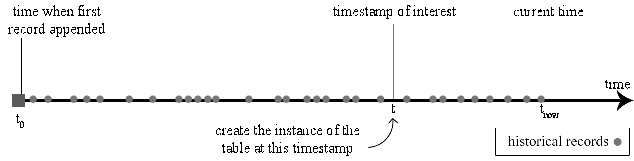
\includegraphics[width=\textwidth]{figs/snapshot_notion.pdf}
	\caption{The notion of creating snapshot on the timeline.}
\end{figure}


\textbf{Proposition. Linear time in creating snapshots}:The notion of creating a snapshot which shows the instance of the table $r$ in a certain timestamp $t$, using historical records stored in an append-only temporal relational table $r^T$ defined in \textbf{Definition 5}. Assume that the tables are updated at a constant rate over time, then the complexity of $\mathrm{snapshot}(r, t)$ is $$\mathcal{O}(|\{x: x\in r^T\mathrm{\ and\ } x.\mathrm{updates} \leq t\}|)\simeq \mathcal{O}(t)$$
Since $r^T$ could be seen as a timeline, the records which needs to be checked can be depicted in \ref{fig:checked_records}. This clearly indicates that a linear time is required to compute a snapshot at a timestamp of interest and as the size of $r^T$ grows in size, creating snapshot become computationally more expensive.

\begin{figure}[b]
	\label{fig:checked_records}
	\centering
	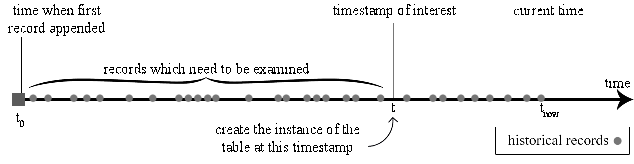
\includegraphics[width=\textwidth]{figs/tobechecked_records.pdf}
	\caption{The records which needs to be checked when creating a snapshot.}
\end{figure}

\textbf{Example.} Given a normal relational table $r_1$ (Table \ref{table:normal_table_2}) and a temporal relational table $r_1^T$ (Table \ref{table:temporal_table_2}) which contains the historical data of $r_1$, the $r_1$ at $t=2018-04-01$ looked like Table $\ref{table:normal_table_2_t}$
\begin{center}

\begin{table}[t]
	\centering
	\caption{Normal Relational Table $r_1$}
	\label{table:normal_table_2}
	\begin{tabular}{p{4cm}p{4cm}p{4cm}}
		\hline
		id & item      & value  \\ \hline
		22 & Pencil    & 7.50 \\
		23 & Notebook & 12.0   \\ 
		24 & Console & 230.0 \\ \hline
	\end{tabular}
\end{table}

\begin{table}[t]
	\centering
	\caption{Temporal Table $r_1^T$}
	\label {table:temporal_table_2}
	\begin{tabular}{p{1cm}p{2cm}p{3cm}p{3cm}p{2cm}}
		\hline
		id & item      & value  & updated  & deleted\\ \hline
		21 & Ruler    & 3.25  & 2018-02-10  &  - \\  
		22 & Pencil    & 8.0  & 2018-03-21  &  - \\
		22 & Pencil    & 9.0  & 2018-03-30  &  -\\
		23 & Notebook & 11.0  & 2018-04-01 & - \\
		22 & Pencil & 6.0  & 2018-04-01 & - \\
		21 & Ruler    & 3.25  & -  &  2018-04-02 \\
		23 & Notebook & 12.0  & 2018-04-02 & - \\ 
		22 & Pencil & 7.50  & 2018-04-05 & - \\ 
		24 & Console & 230.0  & 2018-04-05 & - \\ \hline
	\end{tabular}
\end{table}
\end{center}
\begin{center}
\begin{table}
	\centering
	\caption{Normal Relational Table $r_1$ at t = 2018-04-01}
	\label{table:normal_table_2_t}
	\begin{tabular}{p{4cm}p{4cm}p{4cm}}
		\hline
		id & item  & value  \\ \hline
		21 & Ruler & 3.25 \\
		22 & Pencil & 6.0   \\ 
		23 & Notebook & 11.0 \\ \hline
	\end{tabular}
\end{table}
\end{center}

\subsection{Query answering using snapshots} 

Using precomputed materialized view has been proven to be effective in reducing computational time of query answering \cite{sohrabi2016materialized} \cite{du2017deepsea}. Since running queries $Q(t)$ on temporal table $r^T$ to build snapshots or generate latest version of a record at a timestamp of interest requires linear time with time complexity of approximately $\mathcal{O}(t)$, therefore in the presence of multiple and concurrent queries, such transactions are computationally expensive and inefficient. We argue that, if a snapshot is computed at the timestamp $t$ and placed on the timeline, computational time of answering to the subsequent queries on $r^T$ is reduced. The notion of having precomputed snapshots for materialization can be depicted as Figure \ref{fig:snapshot_materialization}. Note that the snapshot could exist before or after a query and in both cases the query can use the snaphsot for materialization.

\begin{figure}[t]
	\label{fig:snapshot_materialization}
	\centering
	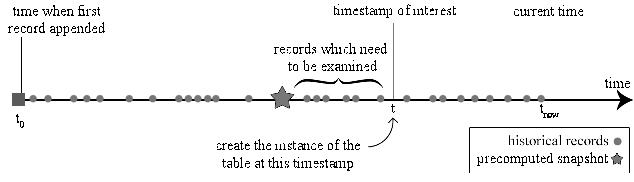
\includegraphics[width=\textwidth]{figs/snapshot_materialization.pdf}
	\caption{The records which needs to be checked when creating a snapshot with having a precomputed snapshot for materialization.}
\end{figure}

\textbf{Proposition} suppose we have a materialized snapshot $snapshot(r,s)$. Then $snapshot(r,t)$ can be computed with complexity:
$$\mathcal{O}(|\{x: x\in r^T\mathrm{\ and\ } x.\mathrm{updates} \in [s,t]\}|) \simeq \mathcal{O}(|s-t|)$$

\textbf{Example.} Given a temporal relational table $r_1^T$ (Table \ref{table:temporal_table_3}) and a precomputed snapshot table $s_1$ at timestamp $t = 2018-03-11$(Table \ref{table:snapshot_s1}), we are interested to create a snapshot $s_2$ which is the instance of table $r_1$ at the timestamp of $t = 2018-03-15$. In order to compute snapshot $s_2$, Table \ref{table:transactions_nonmaterialized} shows the transactions which needs to be evaluated without using snapshot $s_1$ and Table \ref{table:transactions_nonmaterialized} is when $s_1$ is used for materialization. This example clearly shows that when creating snapshot $s_2$ (Table \ref{table:snapshot_s2}), less transactions need to be evaluated when $s_1$ is used for materialization.

\begin{center}
\begin{table}
	\centering
	\caption{Temporal Table $r_1^T$}
	\label {table:temporal_table_3}
	\begin{tabular}{p{1cm}p{2cm}p{3cm}p{3cm}p{2cm}}
		\hline
		id & item & value  & updated  & deleted\\ \hline
		1 & Paper & 0.25  & 2018-02-10  &  - \\  
		2 & Scissors & 8.0  & 2018-02-12  &  - \\
		3 & Folder & 1.50  & 2018-02-12  &  - \\
		1 & Paper & 0.30  & 2018-02-13  &  - \\
		4 & Pencil & 3.0  & 2018-02-16  &  - \\
		3 & Folder & 1.75  & 2018-02-21  &  - \\
		5 & Batteries & 8.0  & 2018-02-23  &  - \\
		1 & Paper & 0.35  & 2018-02-25  &  - \\
		6 & Notebook & 7.0  & 2018-03-01  &  - \\
		5 & Batteries & 9.0  & 2018-03-01  &  - \\
		4 & Pencil & 3.25  & 2018-03-04  &  - \\
		1 & Paper & 0.35  &  - &  2018-03-04 \\
		7 & Ruler & 4.0  & 2018-03-06  &  - \\
		2 & Scissors & 8.50  & 2018-03-07  &  - \\
		7 & Ruler & 4.50  & 2018-03-08  &  -\\
		5 & Batteries & 11.0  & 2018-03-10 & - \\
		3 & Folder & 1.75  & - & 2018-03-11 \\
		7 & Ruler & 4.50  & -  &  2018-03-12 \\
		6 & Notebook & 7.50  & 2018-03-15 & - \\ 
		2 & Scissors & 7.50  & 2018-03-17 & - \\ \hline
	\end{tabular}
\end{table}
\begin{table}
	\centering
	\caption{Snapshot $s_1$ at $t = 2018-03-11$}
	\label{table:snapshot_s1}
	\begin{tabular}{p{4cm}p{4cm}p{4cm}}
		\hline
		id & item  & value  \\ \hline
		2 & Scissors & 8.5   \\ 
		4 & Pencil & 3.25   \\ 
		5 & Batteries & 11.0   \\ 
		6 & Notebook & 7.0 \\ 
		7 & Ruler & 4.50   \\ \hline
	\end{tabular}
\end{table}
\end{center}

\begin{center}
\begin{table}
	\centering
	\caption{the transactions to compute snapshot $s_2$ at $t = 2018-03-15$ without using snapshot $s_1$ for materialization}
	\label{table:transactions_nonmaterialized}
	\begin{tabular}{p{1cm}p{2cm}p{2cm}p{3cm}p{2cm}p{2cm}}
		\hline
		id & item & Transaction  &timestamp & value  &query on\\ \hline
		1 & Paper & cretaed & 2018-02-10 & 0.25 & $r_1^T$ \\
		  & Paper & updated & 2018-02-13 & 0.30 & $r_1^T$ \\
		  & Paper & updated & 2018-02-25 & 0.35 & $r_1^T$ \\
		  & Paper & deleted & 2018-03-04 & - & $r_1^T$ \\ \hline
		2 & Scissors & cretaed & 2018-02-12 & 8.0 & $r_1^T$ \\
		  & Scissors & updated & 2018-03-07 & 8.50 & $r_1^T$ \\ \hline
		3 & Folder & cretaed & 2018-02-12 & 1.50 & $r_1^T$ \\
		  & Folder & updated & 2018-02-21 & 1.75 & $r_1^T$ \\
		  & Folder & deleted & 2018-03-11 & - & $r_1^T$ \\ \hline
	  	4 & Pencil & cretaed & 2018-02-16 & 3.0 & $r_1^T$ \\
		  & Pencil & updated & 2018-03-04 & 3.25 & $r_1^T$ \\ \hline
  	  	5 & Batteries & cretaed & 2018-02-23 & 8.0 & $r_1^T$ \\
		  & Batteries & updated & 2018-03-01 & 9.0 & $r_1^T$ \\
		  & Batteries & updated & 2018-03-10 & 11.0 & $r_1^T$ \\ \hline
		6 & Notebook & cretaed & 2018-03-01 & 7.0 & $r_1^T$ \\ 
		  & Notebook & updated & 2018-03-15 & 7.50 & $r_1^T$ \\ \hline
		7 & Ruler & cretaed & 2018-03-06 & 4.0 & $r_1^T$ \\
		  & Ruler & updated & 2018-03-08 & 4.50 & $r_1^T$ \\
		  & Ruler & deleted & 2018-03-12 & - & $r_1^T$ \\ \hline

	\end{tabular}
\end{table}
\end{center}

\begin{center}
\begin{table}
	\centering
	\caption{the transactions to compute snapshot $s_2$ at $t = 2018-03-15$ using snapshot $s_1$ for materialization}
	\label{table:transactions_materialized}
	\begin{tabular}{p{1cm}p{2cm}p{2cm}p{3cm}p{2cm}p{2cm}}
		\hline
		id & item & Transaction  &timestamp & value  &query on\\ \hline
		2 & Scissors & - & - & 8.50 & $s_1$ \\ \hline
	  	4 & Pencil & - & - & 3.25 & $s_1$ \\ \hline
  	  	5 & Batteries & - & - & 11.0 & $s_1$ \\ \hline
		6 & Notebook & - & - & 7.0 & $s_1$ \\ 
		  & Notebook & updated & 2018-03-15 & 7.50 & $r_1^T$ \\ \hline
		7 & Ruler & - & - & 4.50 & $s_1$ \\
		  & Ruler & deleted & 2018-03-12 & - & $r_1^T$ \\ \hline
	\end{tabular}
\end{table}
\end{center}

\begin{center}
\begin{table}
	\centering
	\caption{Snapshot $s_2$ at $t = 2018-03-15$}
	\label{table:snapshot_s2}
	\begin{tabular}{p{4cm}p{4cm}p{4cm}}
		\hline
		id & item  & value  \\ \hline
		2 & Scissors & 8.50   \\ 
		4 & Pencil & 3.25   \\ 
		5 & Batteries & 11.0   \\ 
		6 & Notebook & 7.50 \\ \hline
	\end{tabular}
\end{table}
\end{center}

\subsection{Optimal materialization of snapshots}
Let $T_q = \{q_1, q_2, \dots, q_n :q_i \in \mathcal{T}\}$ be the timestamps of $n$ queries, each querying the database at $D^T(q_i)$. To save on computational cost in answering the queries on temporal database $D^T$, we propose to compute $m$ number of snapshots $snapshot_j(r,t)$ in optimal timestamps on the timeline to answer to $T_q$ at lowest possible cost. The cost function is defined as the total query answering cost given $m$ number of precomputed snapshots. Note that $m$ is defined based on available resources in the system.

\textbf{Definition. (Cost of Query Answering)}: In the presence of a single materialized precomputed snapshot at timestamp $s \in \mathcal{T}$, the cost of answering the query $T_q$ is calculated as:
$$\mathrm{cost}(T_q | s) = \sum_{q\in T_q} |q - s|$$
Now if multiple snapshots at timestamps $S=\{s_1, s_2, \dots, s_m : s_j \in \mathcal{T}\}$ were precomputed and materialized, then 
$$\mathrm{cost}(T_q|S) = \sum_{q\in T_q} \min\{|q-s| : s\in S\}$$

\textbf{Definition. (Optimal Snapshot placement)}: For the \emph{single snapshot placement} problem, the goal is to find the timestamp $s^*$ such that 
$$cost(T_q|s)= Arg min(\sum_{q\in T_q}|q - s|)$$

The \emph{$m$-snapshot placement} problem is to compute $m$ number of timestamps $S^*=\{s_1, s_2, \dots, s_m: s_j \in \mathcal{T}\}$ to place $m$ number of snapshots for materialization, such that 
$$cost(T_q|S)= Arg min(\sum_{q\in T_q}\{|q - s|:s \in S\})$$

in the subsequent sections, we present the algorithms to address the problem of snapshot placement.

\section{Optimal single snapshot placement}
\textbf{Proposition} Let $T_q^* = {q_1,q_2, \dots , q_n}$ be $n$ number of queries performed on the temporal database. $T_q^*$ gives us a valuable insight into the query patterns on the temporal database, that could be used to find optimal position of snapshots.

\textbf{Proposition}: Given the performed queries $T_q^*$, the optimal position for a single snapshot on the timeline for materialization is $s^*(T_q^*)=median(T_q^*)$ that can be computed in $\mathcal{O}(|T_q^*|)$. Figure \ref{fig:optimal_materialization} shows the notion of placing snapshot in the median of queries for materialization.

\begin{figure}
	\label{fig:optimal_materialization}
	\centering
	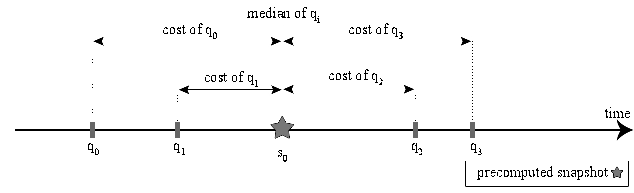
\includegraphics[width=\textwidth]{figs/optimal_materialization.pdf}
	\caption{Placing a single snapshot in the median of queries guarantees the optimal cost of query answering.}
\end{figure}

\textbf{\emph{Proof of the proposition}}:
At first, the placement of a single snapshot for two queries are discussed and then the argument is generalized for multiple queries:\\
Assume that there are two queries $T_q=\{q_1,q_2\ : q_i \in \mathcal{T}\}$ on the timeline, such that, $q_1<q_2$. for the placement of a single snapshot $s^* \in \mathcal{T}$ on the timeline, there are several cases which needs to be considered:\\
\emph{Case 1}:
$s^* \in [q_1,q_2]$, hence $q_1\leq s^*\leq q_2$.
in this case, the cost is:\\
$$cost(T_q|s^*)=\sum_{i=1}^2|q_i-s^*| = (s^*-q_1+q_2-s^*)=(q_2-q_1)$$\\
from above, it is concluded that the cost of running two queries $q_1$ and $q_2$ when snapshot is placed between them, is equal to the deviation between the two queries.\\
\emph{Case 2}:
$s^* \notin [q_1,q_2]$ and $s^* < q_1 < q_2$. for this case the cost could be calculated as follows:
$$cost_T(T_q|s^*)=\sum_{i=1}^2|q_i-s^*| = (q_1-s^*+q_2-s^*)=(q_1+q_2-2s^*) $$$$>(q_1+q_2-2q_1)=(q_2-q_1)$$\\
Therefore we conclude that if the snapshot $s^*$ is placed before queries $T_q$, the cost to perform both queries is greater than when the snapshot is placed between the two queries.\\
\emph{Case 3}:
$s^* \notin [q_1,q_2]$ and $q_1 < q_2 < s^*$.
$$cost(T_q|s^*)=\sum_{i=1}^2|q_i-s^*| = (s^*-q_1+s^*-q_2)=(2s^*-q_1-q_2) $$$$>(2q_2-q_1-q_2)=(q_2-q_1)$$\\
hence, if the snapshot $s^*$ is placed after the queries $T_q$, then the cost of performing those queries are greater than when the snapshot is placed between them.\\
From case1, case2 and case3, we can conclude that the optimal timestamp on the timeline where we can place the single snapshot $s^* \in \mathcal{T}$ to perform two queries $T_q = \{q_1,q_2:q_i\in \mathcal{T}\}$, where $q_1<q_2$ is when $s^* \in [q_1,q_2]$, meaning that $q_1 \leq s^* \leq q_2$, where the cost is equal to $q_2-q_1$.\\

Now, we generalize our conclusion from the cases that we evaluated, for the placement of a single snapshot in the presence of $n$ number of queries on the timeline: 

Suppose that there is a set of queries $T_q=\{q_1,q_2,...,q_n:q_i \in \mathcal{T}\}$ performed on the timeline. To evaluate the most optimal position to place the single snapshot $s^* \in \mathcal{T}$ for materialization, we breakdown the set of queries into the set of nested intervals $[q_1,q_n],[q_2,q_{n-1}],...,[q_i,q_{n+1-i}]$ where $n$ is the number of queries on timeline and $i=0,1,2,...,c$ where $c=\frac{n+1}{2}$ when there are odd number of queries and $c=\frac{n}{2}$ when there are even number of queries present on the timeline.\\ 
Based on the conclusion that we obtained from examining case 1, case 2 and case 3 earlier, for each nested interval, the cost of queries inside them is minimized if snapshot $s^*$ is placed in a middle of the interval. Therefore if the snapshot is placed in a position which $s^*\in \{ [q_1,q_n] \wedge [q_2,q_{n-1}] \wedge ... \wedge [q_i,q_{n+1-i}] \}$ the overall cost for all queries is minimized. In other words, if the snapshot is placed in a position that is in the middle of all nested intervals, then the total sum of absolute deviation of the snapshot from all queries is minimized. The placement of snapshot $s^*$ in the median position of $T_q$, guarantees that the snapshot is placed in the middle of all nested query intervals, where the cost of queries is calculated as follows:
$$cost(T_q|s^*)=\sum_{i=1}^n |q_i-s^*| = $$
$$[(|q_1-s^*|+|q_n-s^*|)+(|q_2-s^*|+|q_{n-1}-s^*|)+...+|q_c-s^*|+|q_{n+1-c}-s^*|)]=$$
$$[(s^*-q_1+q_n-s^*)+(s^*-q_2+q_{n-1}-s^*)+...+(s^*-q_c+q_{n+1-c}-s^*)]=$$
$$[(q_n-q_1)+(q_{n-1}-q_2)+...+(q_{n+1-c}-q_c)]$$\\
where parenthesis indicate the deviation from endpoints for one of nested intervals. In the case when there are odd number of queries performed on the timeline, the innermost interval is $[q_{\frac{n+1}{2}},q_{\frac{n+1}{2}}]$ and the position of $q_{\frac{n+1}{2}}$ is the optimal position to place snapshot $s^*$. also when there are even number of queries the innermost interval is $[q_{\frac{n}{2}},q_{\frac{n}{2}+1}]$, therefore if we choose snapshot $s^*$'s position to be at $q_{\frac{n}{2}}\leq s^*\leq q_{\frac{n}{2}+1}$,it guarantees that the snapshot exists inside each of nested intervals, and hence the sum of absolute deviation is minimized. \\

\section{Optimal multiple snapshot placement}
In the presence of thousands of queries on a temporal database with millions of records, having a single snapshot reduces the cost of query answering but it is still not enough. Therefore, to reduce the overall cost of query answring, optimal timestamps should be computed on the timeline of the temporal database to place snapshots for materialization. In the following section, different approaches to compute the optimal positions on the timeline are discussed.

\textbf{\emph{Proposition (Segmentation of queries)}}: Given an ordered set of snapshot timestamps $S=\{s_1,s_2,...,s_m:s_i \in \mathcal{T}\}$, such that $s_i \leq s_{i+1}$, and $n$ number of queries $Q = \{q_1,q_2,...,q_n: q_i \in \mathcal{T}\}$, snapshots create $m$ number of non-overlapping segments on the queries $Q[1,i_1],Q[i_1+1,i_2],...,Q[i_{m-1},i_m]$ such that queries in the segment $Q[i_j,i_{j+1}]$ use $s_j$ to answer the queries in the optimal query answering strategy. The notion of creating segmentations is depicted in Figure \ref{fig:segmentation}.

\begin{figure}
	\label{fig:segmentation}
	\centering
	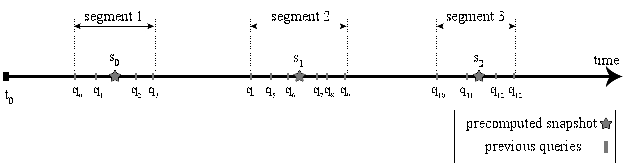
\includegraphics[width=\textwidth]{figs/segmentations.pdf}
	\caption{The notion of creating segmentations on the timeline and placing snapshot for each segmentation.}
\end{figure}

\subsection{A recursive algorithm for optimal snapshot placements}

Let $\mathrm{opt}(Q, m)$ be the optimal $m$-snapshot placements for the query workload $Q$. Denote $Q[i,j] = \{q_i,q_{i+1},...,q_{j-1},q_j\}$.

\textbf{\emph{Proposition. (Optimality of sub-problems)}}
Let $S^* = \mathrm{opt}(Q, m)$.  Let $\mathcal{Q}$ be the partition of segments created by $S^*$.  Then, the prefix of $S^*$ is also an optimal $m-1$ snapshot placement of the prefix of $\mathcal{Q}$. Formally, $$\mathrm{prefix}(S^*) = \mathrm{opt}(\cup\mathrm{prefix}(\mathcal{Q}), m-1)$$
We can formulate a recursive definition of $\mathrm{opt}(Q, m)$ using
Proposition~\ref{thm:subopt}.  The intuition is that we try out all possible
{\em last} segment of $Q$, and pick the one with the lowest cost.

The recursive definition of $\mathrm{opt}(Q, m)$ is given as:

\begin{itemize}
	\item Base case $ \mathrm{opt}(Q, 1) = \{\mathrm{median}(Q)\}$.
	\item Induction on $m$:
	$$i^* = \mathrm{argmin}\{\mathrm{cost}(\mathrm{opt}(Q[1,i], m-1)): i\in[1,
	n]\}$$
	$$
	\mathrm{opt}(Q, m) = \mathrm{opt}(Q[1, i^*]) \cup \{\mathrm{median}(Q[i^*+1, n])
	$$
\end{itemize}
The recursive formulation of $\mathrm{opt}(Q, m)$ requires $\mathcal{O}(2^{m})$.

\subsection{Dynamic programming approach to optimal snapshot placements}

We can build a table $\mathbf{OPT}$ as a two dimensional array
indexed by $(i, k)$ where $i\in [1, n]$ and $k\in [1, m]$.  Each entry
in the table $\mathbf{OPT}[i,k] = \mathrm{opt}(Q[1,i], k)$.
We can compute $\mathbf{OPT}[i,k]$ in a bottom up fashion \cite{}.

\vspace{1em}
{\small
	\begin{tabular}{|l|} \hline
		computeOPT($Q$, $m$) = \\
		\verb|| $n = |Q|$ \\
		\verb|| $\mathbf{OPT}[i, 0] = \infty$ \\
		\verb|| for $k = 1 \to m$ \\
		\verb| | for $i = 1 \to n$ \\
		\verb|  | $j^* = \underset{j\in[1,i]}{\mathrm{argmin}}
		(\mathrm{cost}(\mathbf{OPT}[j,k-1]) + \mathrm{cost}(Q[j+1, n]))$ \\
		\verb|  | $\mathbf{OPT}[i,k] = \mathbf{OPT}[j^*, k-1] \cup \{\mathrm{median}(Q[j+1], n)\}$ \\
		\verb| | end for \\
		\verb|| end for \\ \hline
	\end{tabular}
}
\vspace{1em}

\textbf{\emph{proposition.}} The complexity of computing all the entries of $\mathbf{OPT}$ is $\mathcal{O}(mn^2)$.

\subsection{Heuristic snapshot placements}

\section{Discussion}
